% \documentclass[rnd]{mas_proposal}
\documentclass[thesis]{mas_proposal}

\usepackage[utf8]{inputenc}
\usepackage{amsmath}
\usepackage{amsfonts}
\usepackage{amssymb}
\usepackage{graphicx}

\title{Project Proposal Title}
\author{Lokesh Veeramacheneni}
\supervisors{Dr. Paul G Pl\"{o}ger\\ Dr. Matias Valdenegro Toro \\ Third Supervisor}
\date{Month 2021}

% \thirdpartylogo{path/to/your/image}

\begin{document}

\maketitle

\pagestyle{plain}

\section{Introduction}
\begin{itemize}
    \item An introduction to the general topic you are covering.
    \item Why is it important?
\end{itemize}

\subsection{Problem Statement}
\begin{itemize}
    \item What are you going to solve?
    \item How are you evaluating?
\end{itemize}


\section{Related Work}
\begin{itemize}
    \item What have other people done?
    \item Why is it not sufficient?
\end{itemize}

\subsection{Subsection 1}
\subsection{Subsection 2}



\section{Project Plan}

\subsection{Work Packages}
The bare minimum will include the following packages:
\begin{enumerate}
    \item[WP1] Literature Search
    \item[WP2] Experiments
    \item[WP3] Project Report
\end{enumerate}
Keep in mind that depending on your project, you will probably need to add work packages that are more suited to your projects.

\subsection{Milestones}
\begin{enumerate}
    \item[M1] Literature search
    \item[M2] Experimental setup
    \item[M3] Experimental Analysis
    \item[M4] Report submission
\end{enumerate}

\subsection{Project Schedule}
Include a gantt chart here. It doesn't have to be detailed, but it should include the milestones you mentioned above.
Make sure to include the writing of your report throughout the whole project, not just at the end.

\begin{figure}[h!]
    \caption{}
    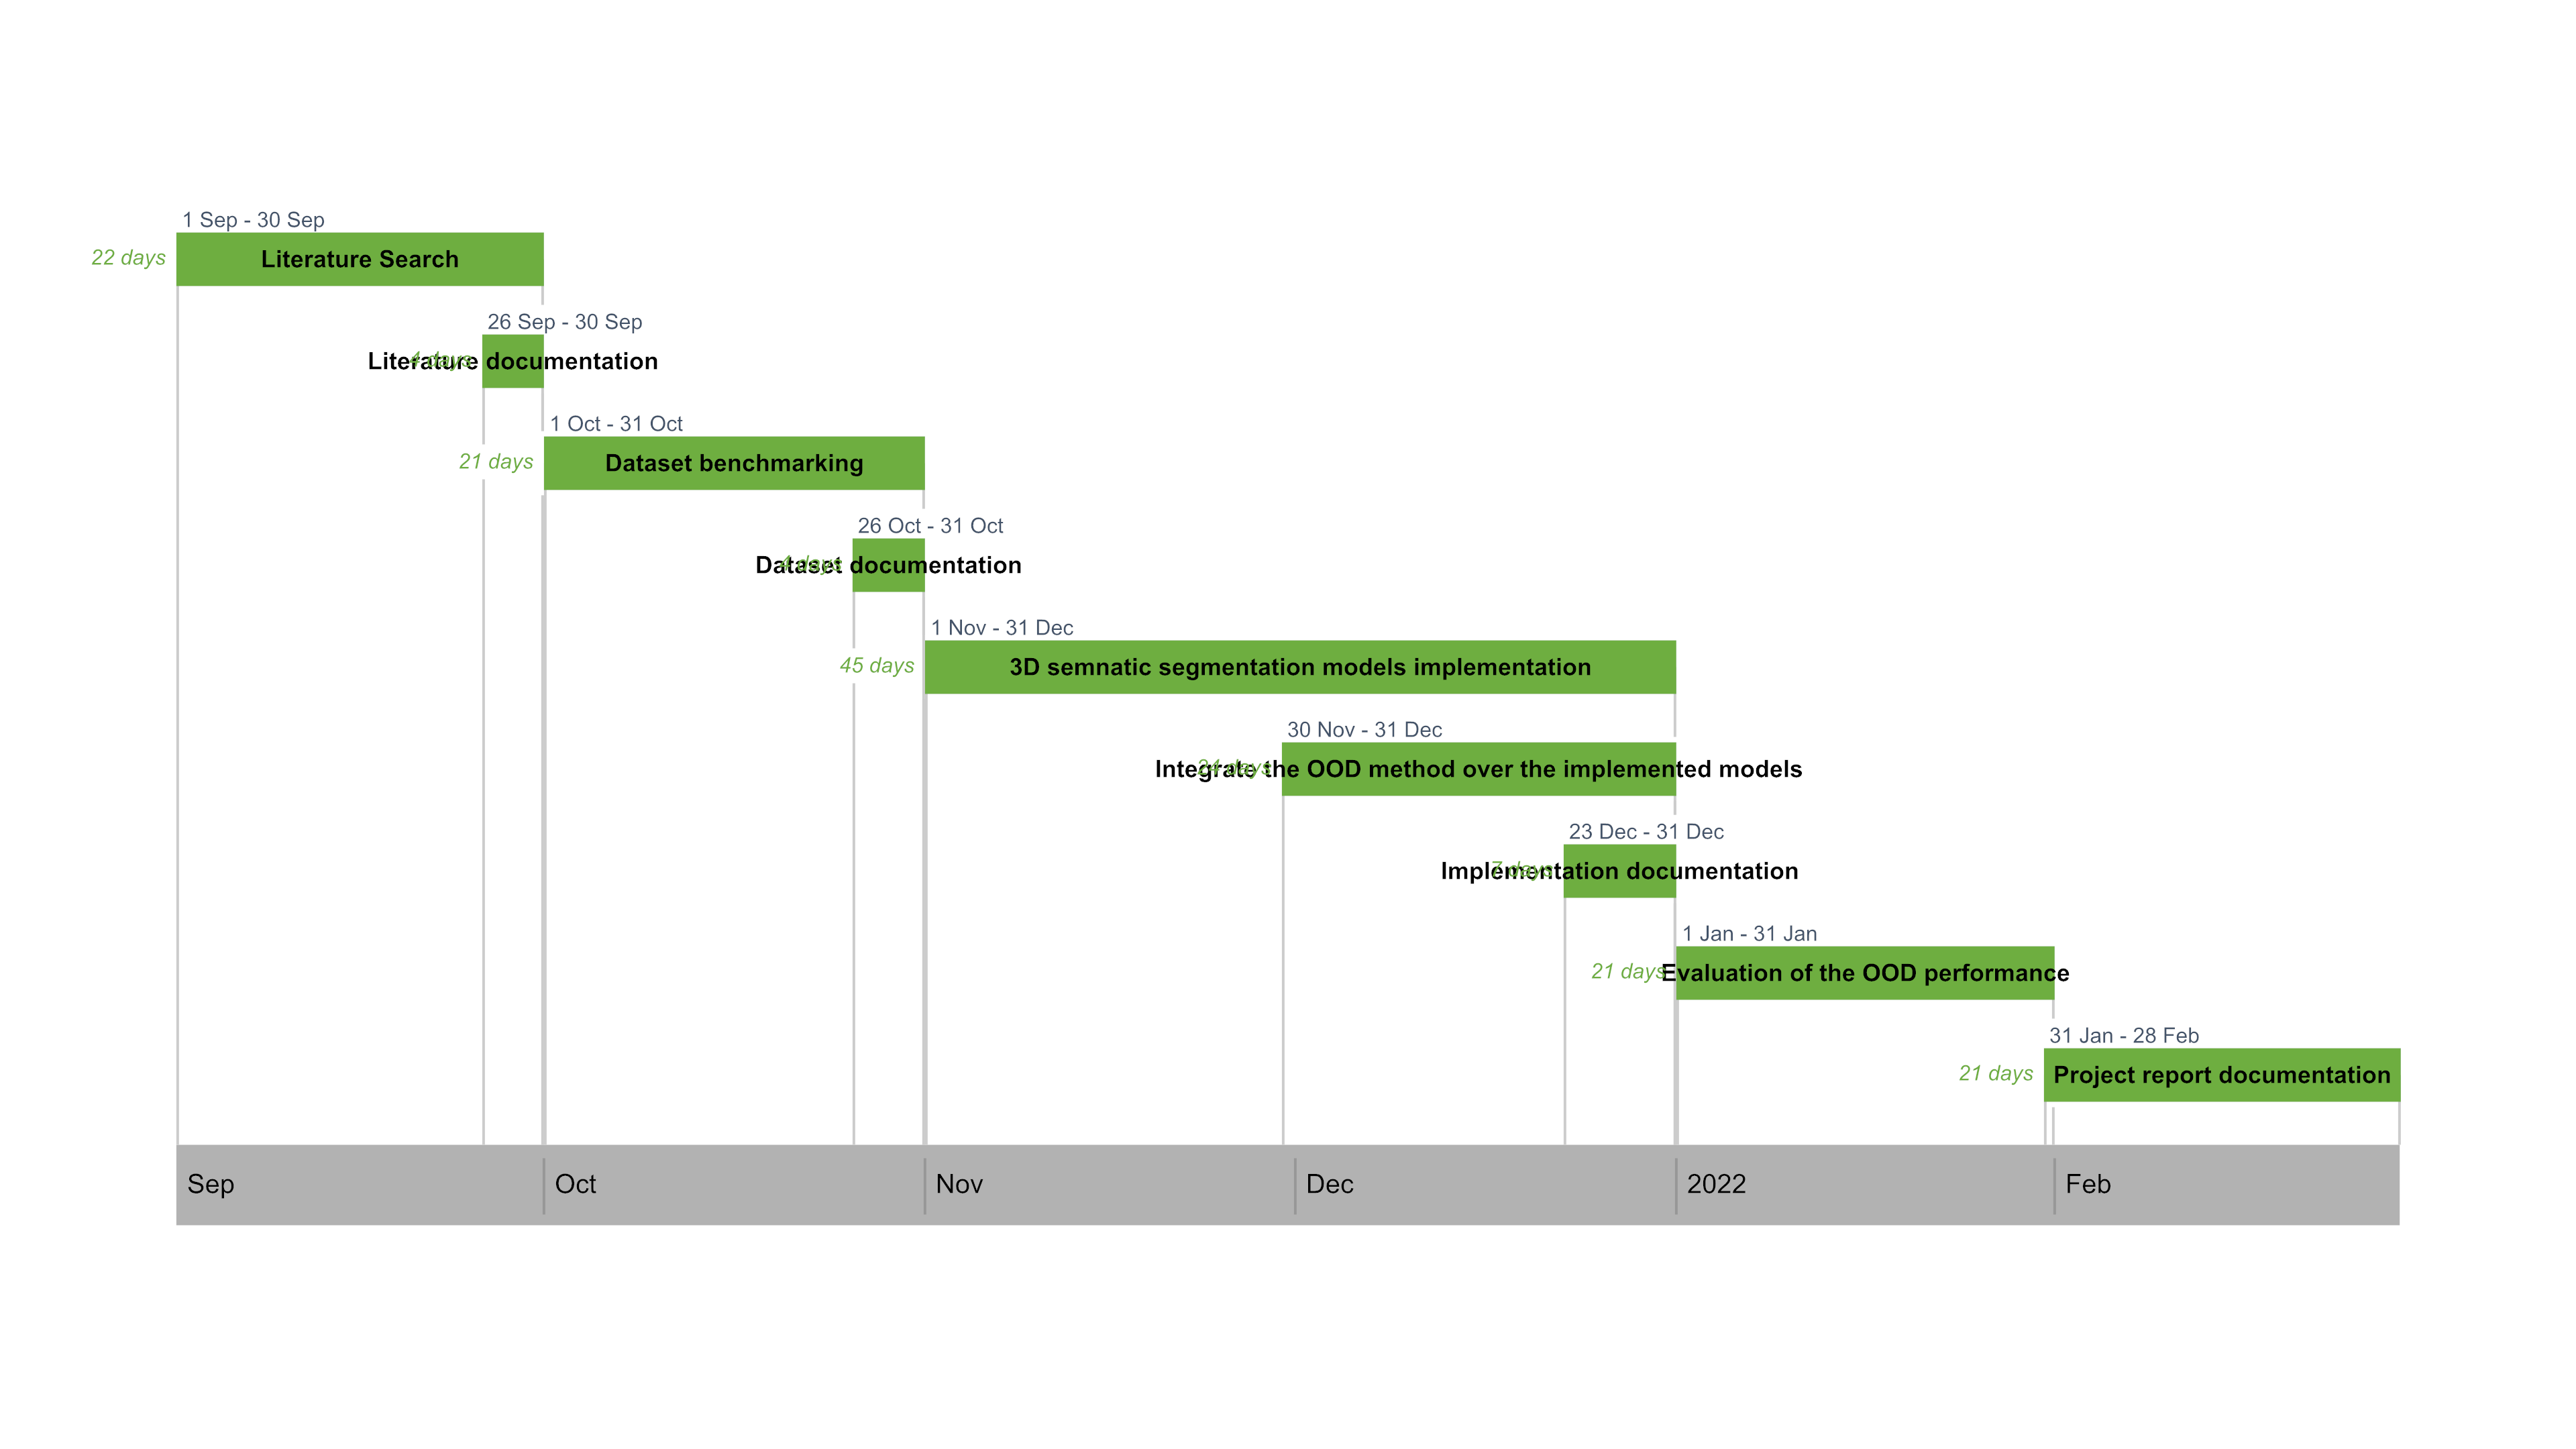
\includegraphics[width=\textwidth]{images/rnd_deliverable_timeline}
    \label{}
\end{figure}

\subsection{Deliverables}
\subsubsection*{Minimum Viable}

\begin{itemize}
    \item Systematic literature survey of methods over
        \subitem- Datasets in 3D LiDAR semantic segmentation
        \subitem- Existing out of distribution methods 
        \subitem- 3D models for semantic segmentation on LiDAR data
    \item Proposal of 3D benchmarking datasets for out of distribution detection
    \item Study of uncertainty estimation over 3D models for OOD detection
    \item Extension of OOD detection method to a baseline 3D model
\end{itemize}

\subsubsection*{Expected}
\begin{itemize}
    \item Systematic evaluation of the implemented baseline model over the benchmarked dataset
    \item Implementation of the state of the art model for OOD detection
    \item Evaluation and comparison of the implemented state of the art model to baseline algorithm
\end{itemize}

\subsubsection*{Desired}
\begin{itemize}
    \item Proposal of a refinement over the current OOD model for higher performance
\end{itemize}


\nocite{*}

\bibliographystyle{plainnat} % Use the plainnat bibliography style
\bibliography{bibliography.bib} % Use the bibliography.bib file as the source of references




\end{document}
